\problem{}

\subproblem{}
\begin{figure}[H]
	\centering
	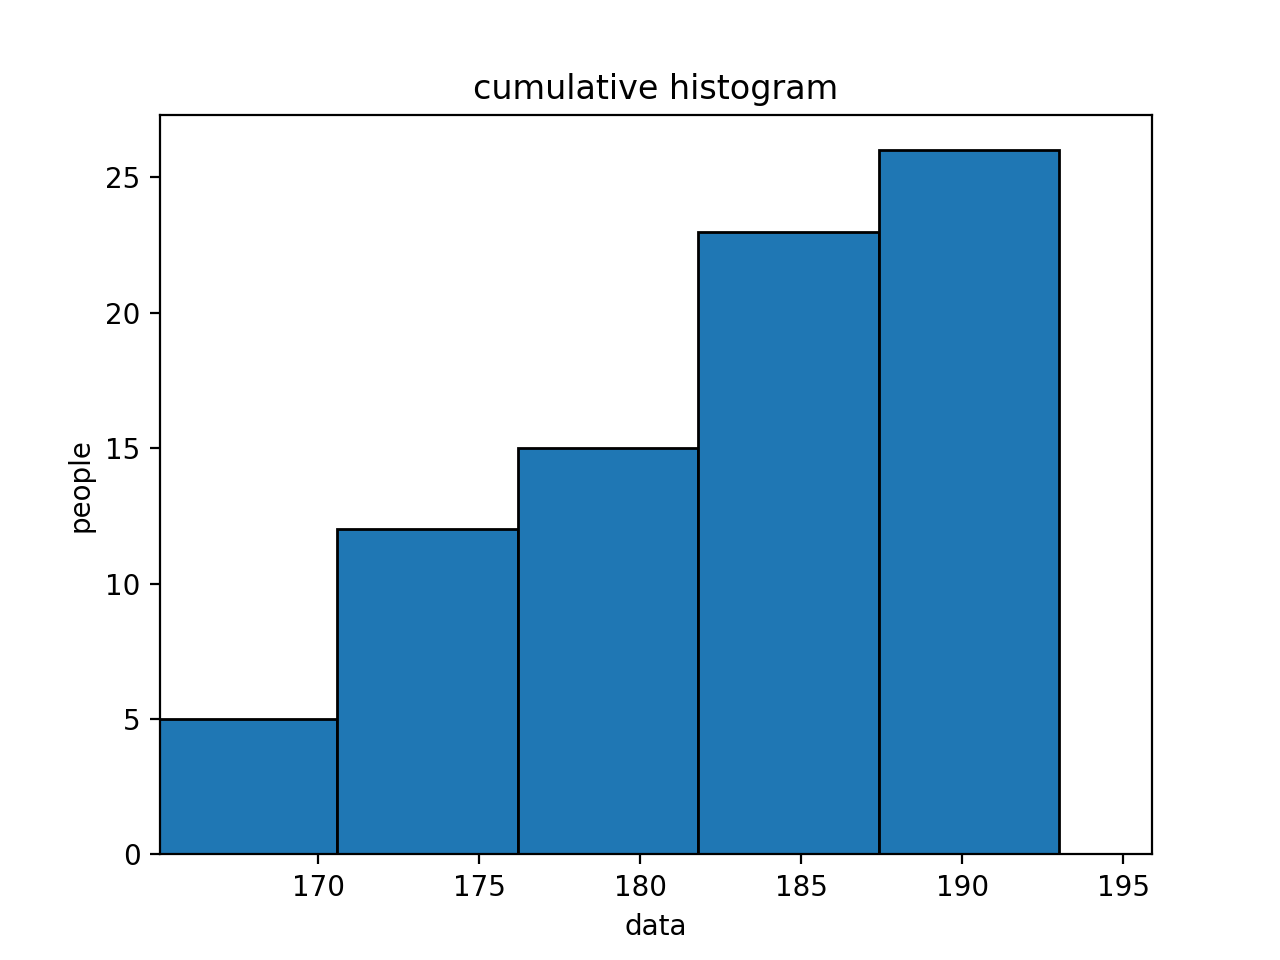
\includegraphics[width=0.5\textwidth]{/Users/kajal/Documents/statistics/resources/hw1/Figure_1.png}
	\caption{نمودار توزیع تجمعی رسم شده توسط python}
\end{figure}

\subproblem{}
برای به دست اوردن میانگین کافیست مقدار مرکز دسته ها را محاسبه کنیم و برای هر دسته مقدار مرکز دسته را در فراوانی نسبی دسته
ضرب کنیم و در نهایت با هم جمع کنیم.
\newline
\newline
\[ \bar{X} = \frac{4 * 167.5 + 5 * 172.5 + 3 * 177.5 + 7 * 182.5 + 5 * 187.5 + 2 * 192.5}{26} = 179.423 \]
\newline
\newline
حالا برای پیدا کردن میانه کافیست با ببینیم در نمودار کدام دسته است که دسته قبل از آن کمتر از $13$ و دسته بعد از آن بیشتر از $13$ فراوانی تجمعی دارد.
که با توجه به شکل دسته $180$ تا $185$ دسته مورد نظر ماست که ابتدای دسته $12$ و انتهای آن $19$ است و با قضیه تالس به سادگی مشخص میشود که اگر یک خط از نقطه $(180,12)$ و $(185,19)$ رد کنیم
در نقطه $180 + \frac{5}{7}$ یعنی تقریبا $180.71 $میانه ما به دست می آید.
که نسبت تالس به صورت زیر است:\newline
\begin{figure}[H]
	\centering
	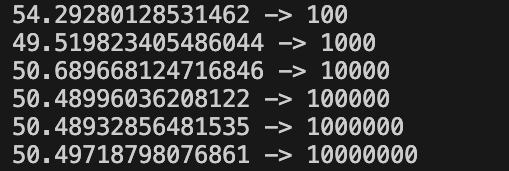
\includegraphics[width=0.5\textwidth]{/Users/kajal/Documents/statistics/resources/hw1/Figure_4.png}
	\caption{پیدا کردن میانه در نمودار هیستوگرام به کمک روش تالس}
\end{figure}

\subproblem{}
اعداد به دست آمده توسط پایتون به صورت زیر هستند که دقیقا با رابطه گفته شده در کلاس
یکی هستند.

\[ Mean Root for -1: 178.201273382513\]
\[Geometric Mean: 178.37000921518623\]
\[Mean Root for 1: 178.53846153846152\]
\[Mean Root for 2: 178.7064632295094\]
